\chapter{Aufwandsschätzung}

\section{Grundlagen}

Die Aufwandsschätzung ist ein kritischer, schwieriger und wichtiger Punkt in der Projektvorbereitung, -vereinbarung und -planung. Sie wird üblicherweise von sämtlichen Vertragsparteien unabhängig durchgeführt. Die Aufwandsschätzung bildet eine Grundlage für die Wirtschaftlichkeit, die Planung von Zeit und Projektmitteln und die Festlegung des erforderlichen Budgets. Der Projekterfolg hängt massgeblich von der Zuverlässigkeit der jeweiligen Schätzungen ab. 
Das Ziel von Schätzungen ist eine realistische Angabe über den erwartenden Aufwand und das erforderliche Budget zu machen.

Pessimistische Schätzungen sind oftmals wirtschaftlich uninteressant, da das Angebot nicht konkurrenzfähig ist. Sie beinhalten die Befürchtungen, dass Mittel und Freiräume dennoch ausgeschöpft werden (?).

Optimistische Schätzungen beinhalten ein grosses Risiko, da das Projekt meist nicht plangemäss durchgeführt werden kann. Sie können zu wirtschaftlichen Verlusten führen.

Aufwand- und Kostenabschätzung sollten sich am Umfang und der Besonderheiten des zu entwickelnden Ergebnisses orientieren. Dies kann die Software selbst, Dokumentation sowie Schulungsunterlagen sowie Dienstleistungen für Schulungen und Unterstützung bei der Einführung sein.

\textbf{Prinzipien bei Schätzungen}
\begin{itemize}
	\item Bildung von Schätzpaketen
	\item Aufwandseinheiten
	\item Einbindung der Mitarbeiter
	\item Dokumentation
	\item Erfahrungswerte und Aufschläge
	\item Kontinuierliche Kontrolle
\end{itemize}


\subsection{Schätzungsansätze}

\begin{minipage}{8cm}
	Aktivitätsorientierte Schätzung
\end{minipage}
\begin{minipage}{7cm}
	Artefaktbasierte Schätzung
\end{minipage}

\begin{figure}[ht]
	\centering
	\adjustbox{width=\textwidth}{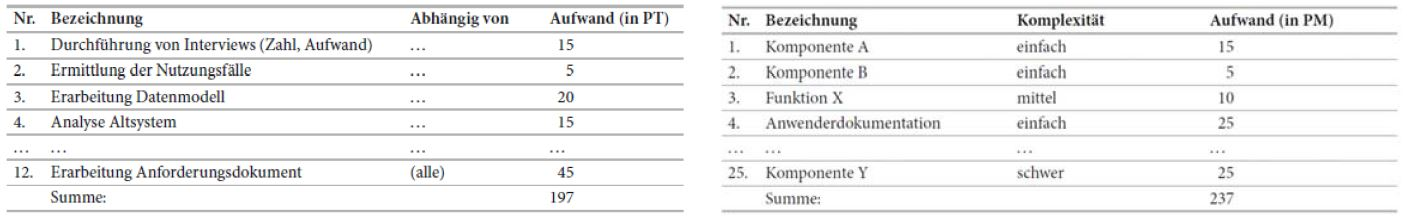
\includegraphics{Figures/schaetzungsansaetze}}
\end{figure}

\subsection{Streuung der Schätzung}

\begin{minipage}{8cm}
	Einflussfaktoren
\end{minipage}
\begin{minipage}{7cm}
	Leistungen in Abhängigkeit des Einsatzes
\end{minipage}

\begin{figure}[ht]
	\centering
	\adjustbox{width=\textwidth}{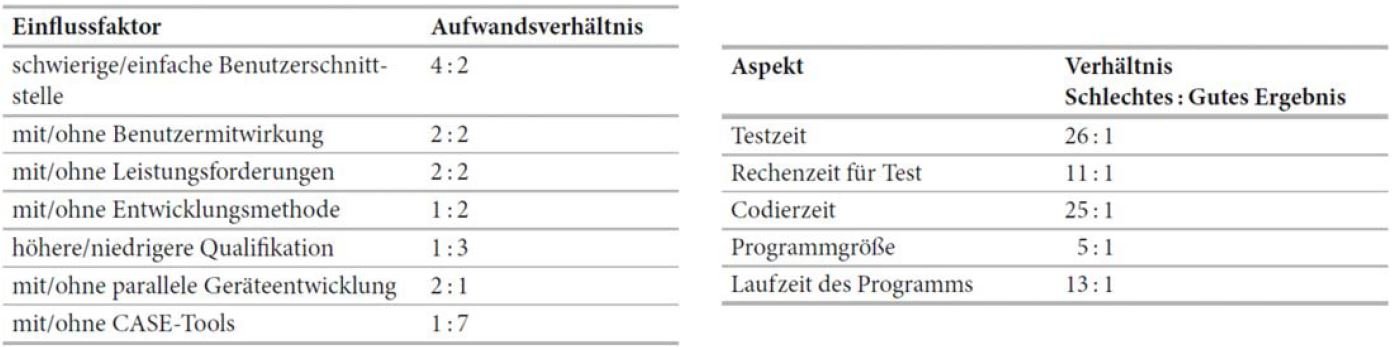
\includegraphics{Figures/streuung}}
\end{figure}

\section{Expertenschätzungen}
Die Expertenschätzungen finden an einer Schätzklausur statt. Dabei führen alle Beteiligten die Schätzung gemeinsam durch. Das Ziel ist dabei realistische Schätzergebnisse mit hoher Genauigkeit unter Berücksichtigung aller relevanten Faktoren zu erzielen. Ausserdem verspricht man sich dabei eine hohe Akzeptanz bei den späteren Projektmitarbeitern. 

\begin{minipage}{8cm}
	\textbf{Delphi Methode}
\end{minipage}
\begin{minipage}{7cm}
	\textbf{Planning Poker}
\end{minipage}

\begin{figure}[hb]
	\centering
	\adjustbox{width=0.49\textwidth}{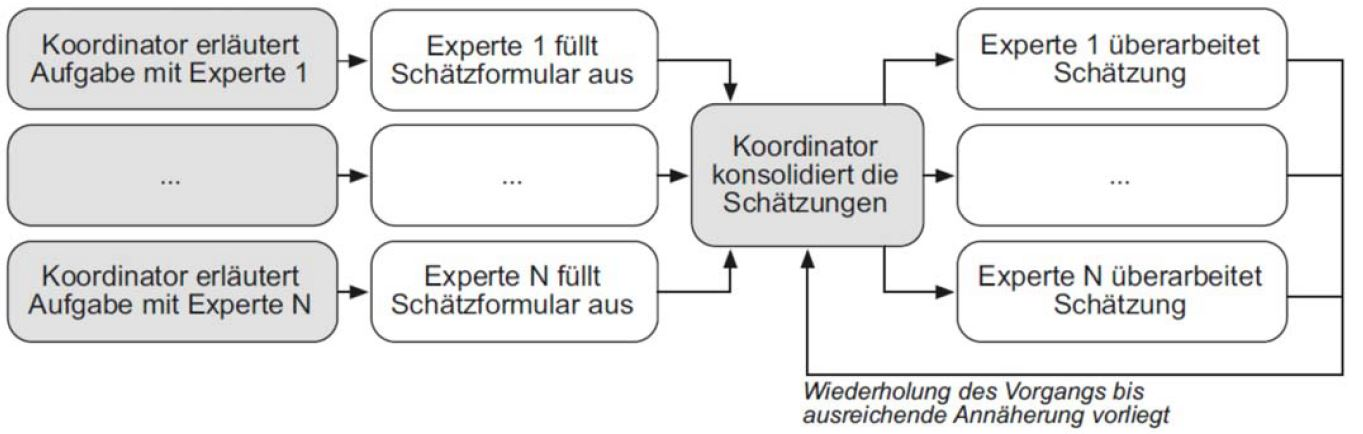
\includegraphics{Figures/delphimethode}}
	\adjustbox{width=0.49\textwidth}{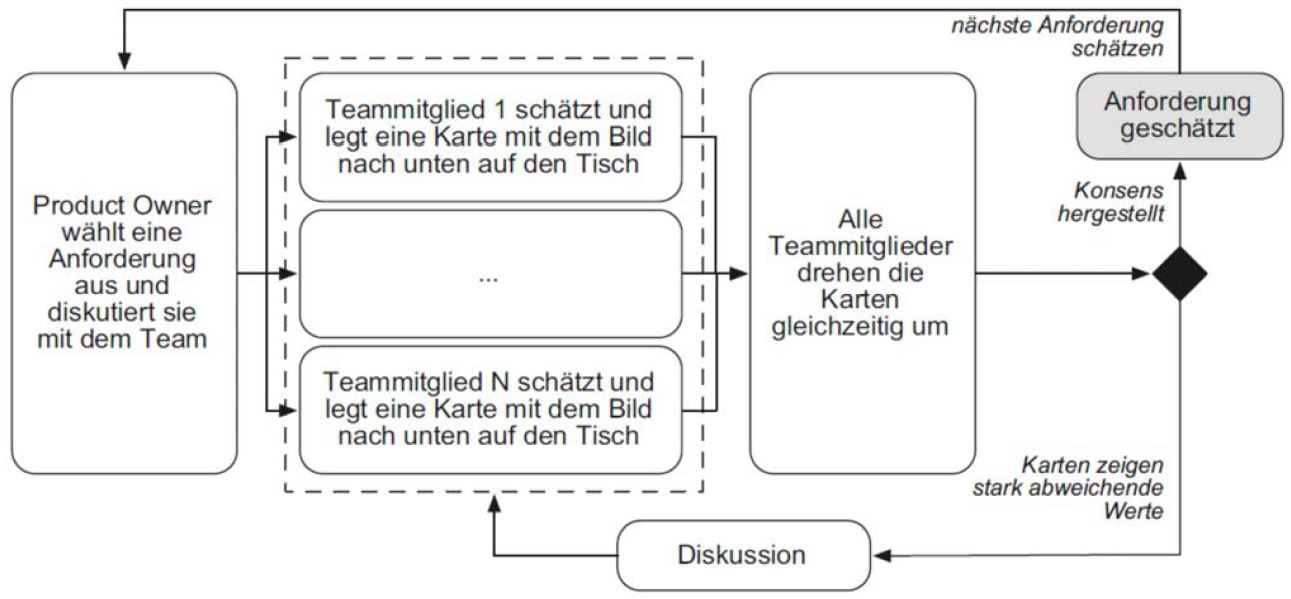
\includegraphics{Figures/planningpoker}}
\end{figure}

\subsection{Drei-Zeiten-Methode (nach PERT) zur Gewichtung von Schätzungen}

Aufwandsmittelwert für Schätzobjekt i: $A_i = \frac{bc_i + 4 lc_i + wc}{6}$ \\
Standardabweichung für Schätzobjekt i: $S_i = \frac{wc_i - bc_i}{6}$ \\
bc: optimistische Schätzung (best case) \\
wc: pessimistische Schätzung (worst case) \\
lc: wahrscheinliche Schätzung (most likely case) 

\section{Algorithmische Schätzverfahren}

\begin{itemize}
	\item Aron-Modell: (Selbststudium) Broy Kap. 6.3.3.1
	\item COCOMO: (Selbststudium) Broy Kap. 6.3.3.2, Hummel Kap. COCOMO S. 70 ff
	\item COCOMO II: (Selbststudium) Broy Kap. 6.3.3.2, Hummel Kap. COCOMO S. 70 ff
	\item Lines of Code (LOC)
	\item Function Points
	\item Speziell für Embedded: 3D Function Points oder COSMIC Full Function Points
\end{itemize}

\subsection{Function Points}
Function Points dienen der Schätzung des Umfangs der geforderten Funktionalität. Die zu schätzende Software wird als Black Box betrachtet, weshalb die Schätzung über die Schnittstellen, mit denen das System mit seiner Umwelt interagiert, erfolgt. 

\textbf{Datenelemente}
\begin{itemize}
	\item (ILF): Internal Logical Files
	\item (ELF): External Interface Files
	\item Data Element Types (DET): für den Systembenutzer sichtbare Datenfelder (z.B. Attribute von Klassen)
	\item Record Element Types (RET): Mehrere logisch zusammenhängende DETs ergeben einen RET
\end{itemize}
DETs und RETs sind verfeinernde Elemente für ILFs und EIFs.

\newpage

\textbf{Transaktionselemente}:
\begin{itemize}
	\item External Input (EI): von dem Benutzer oder einer umgebenden Applikation an die zu schätzende Applikation
	\item External Output (EO): von der zu schätzenden Applikation an den Benutzer oder eine umgebende Applikation
	\item External Query (EQ): Abfrage zwischen Benutzer oder umgebende Applikation und der zu schätzenden Applikation
\end{itemize}

\begin{figure}[hb]
	\centering
	\adjustbox{width=12cm}{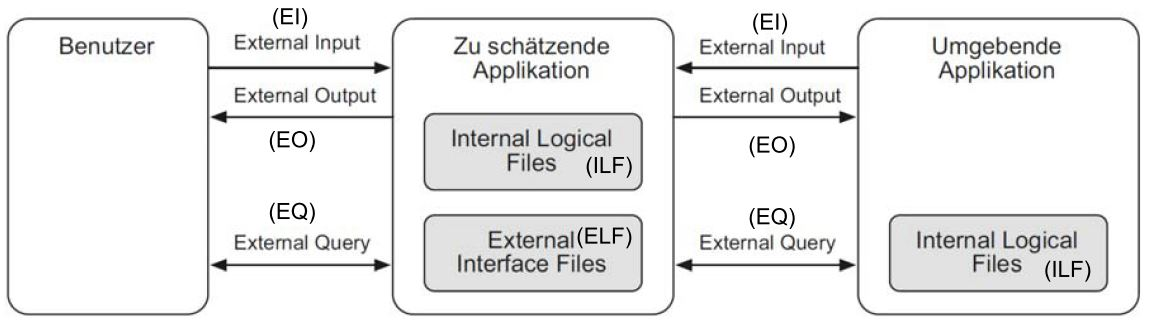
\includegraphics{Figures/transaktionselemente}}
	\caption[]{Daten- und Transaktionselemente}
\end{figure}

\subsubsection{Vorgehen}
Voraussetzung: Die Anforderungen müssen bekannt sein (unabhängig vom Detaillierungsgrad)
\begin{enumerate}
	\item Use-Case Diagramm erstellen: Festlegen der Systemgrenze
	\item Identifikation der Datenelemente (ILF, EIF)
	\item Identfikation der Transaktionselemente (EI, EO, EQ) 
	\item Berechnung der Unadjusted Function Points
\end{enumerate}


\subsubsection{Beispiel zu den Function Pointers}
\begin{figure}
	\centering
	\adjustbox{width=8cm}{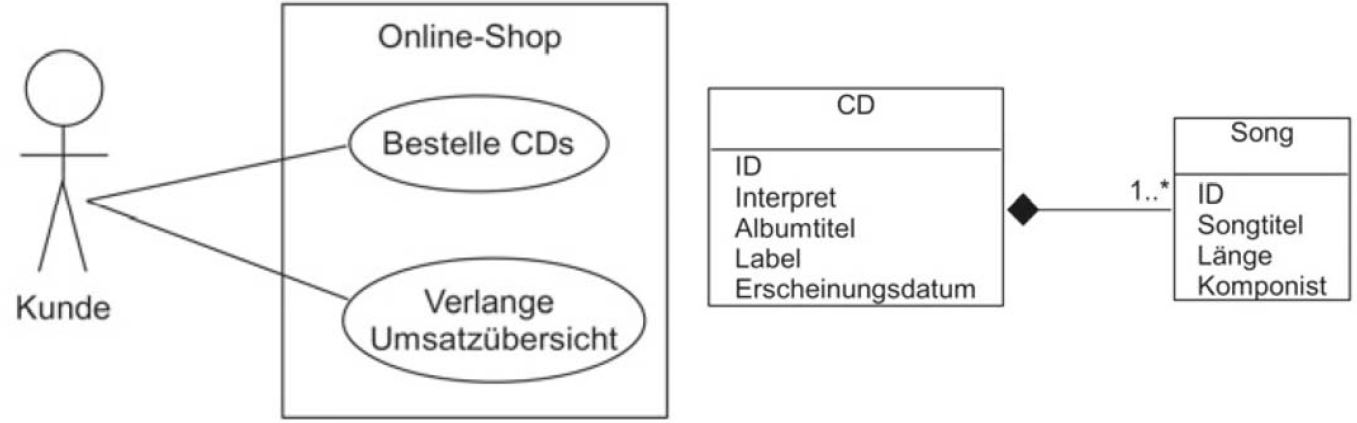
\includegraphics{Figures/fp1}}
\end{figure}
\newpage

\begin{multicols}{2}

\adjustbox{width=0.49\textwidth}{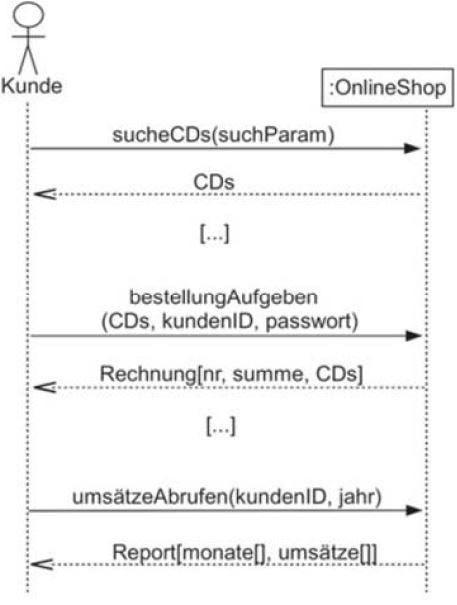
\includegraphics{Figures/fp2}}

\columnbreak
\textbf{Datenelemente} \\
Internal Logical File (ILF): \\
CD; 2 RETs (CD+Song) \\
- CD hat 5 DETs (Attribute von CD) \\
- Song hat 4 DETs (Attribute von Song) \\
DET total: 5+4 DETs (CD + Song)\\
Function Point Rating (FTRs): gering \\
\textbf{Transaktionselemente} \\
- sucheCDs (EQ): 1 FTR (CD), 7 DETs (alle CD Attribute + PushBtn click + Parameter) => geringe Komplexität = 3 FP \\
- bestellungAufgeben (EI): 4 FTR (Kunde, CD, Bestellung, Rechnung), 6 DETs (CD-ID, KundenID, Passwort, PushBtn click, RechnungsNr, Rechnungssumme) => hohe Komplexität: 6 FP \\
- umsätzeAbrufen (EO): 2 FTR(Kunde, Rechnung), 5 DETs(KundenID, Jahr, Monate, Umsätze, PushBtn click) => geringe K.: 4 FP	
\end{multicols}

\subsection{Bewertungslisten}

\begin{minipage}{8cm}
	\textbf{Funktionpoints pro Komplexitätsstufe}
\end{minipage}
\begin{minipage}{7cm}
	\textbf{Komplexität pro Anzahl RETs \& DETs}
\end{minipage}

\begin{figure}[hb]
	\centering
	\adjustbox{width=7cm}{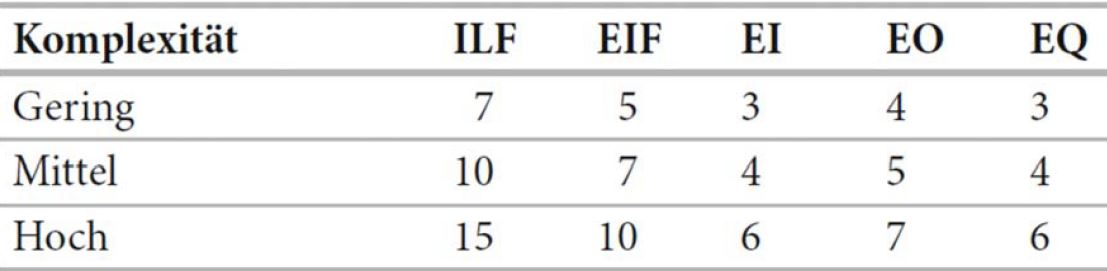
\includegraphics{Figures/Komplexitaet}}
	\adjustbox{width=7cm}{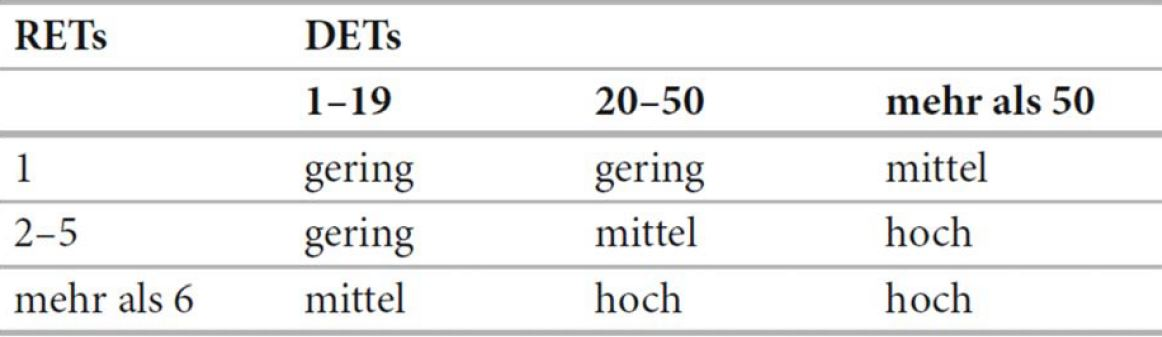
\includegraphics{Figures/RTSDET}}
\end{figure}

\begin{minipage}{8cm}
	\textbf{Function Points Ratings für EI}
\end{minipage}
\begin{minipage}{7cm}
	\textbf{Function Points Ratings für EO und EQ}
\end{minipage}

\begin{figure}[hb]
	\centering
	\adjustbox{width=7cm}{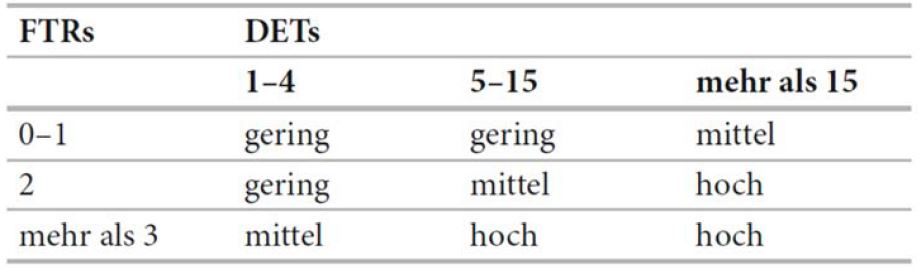
\includegraphics{Figures/FRRfuerEI}}
	\adjustbox{width=7cm}{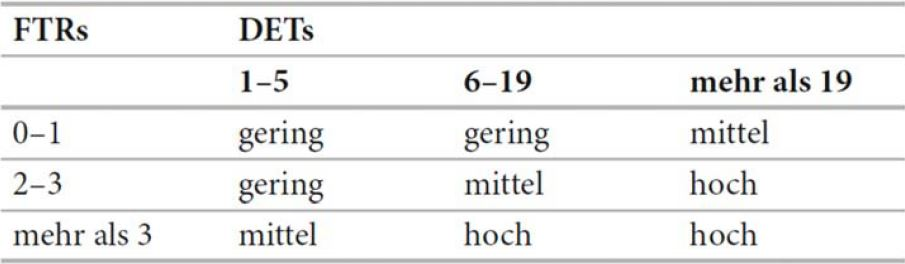
\includegraphics{Figures/FTRfuerEOEQ}}
\end{figure}


\section{Aron (Selbststudium), Broy Kap. 6.3.3.1}

\section{COCOMO (Selbststudium), Broy Kap. 6.3.3.2, Hummel Kap. COCOMO S. 70 ff}

\section{COCOMO II (Selbststudium), Broy Kap. 6.3.3.2, Hummel Kap. COCOMO S. 70 ff}